\documentclass[11pt,a4paper]{article}
\usepackage[T1]{fontenc}
\usepackage[utf8]{inputenc}
\usepackage{lmodern}
\usepackage{amsmath,amssymb,amsthm,mathtools,mathrsfs}
\usepackage{graphicx,float,xcolor,multicol}
\usepackage[shortlabels]{enumitem}
\usepackage[margin=27mm]{geometry}
\usepackage{microtype,needspace,placeins}
\usepackage{tikz,tikz-cd}
\usetikzlibrary{arrows.meta,calc,positioning,patterns,decorations.pathreplacing}
\usepackage[colorlinks=true,linkcolor=teal,urlcolor=teal,citecolor=teal]{hyperref}
\setlength{\parindent}{0pt}
\setlength{\parskip}{.6em}
\setcounter{secnumdepth}{0}
\allowdisplaybreaks
\raggedbottom
\providecommand{\cross}{\times}
\DeclareUnicodeCharacter{2020}{\ensuremath{\dagger}}
\DeclareMathOperator{\supp}{supp}
\DeclareMathOperator*{\esssup}{ess\,sup}
\providecommand{\chapter}{\section}
\newenvironment{tool}[2]{\subsection*{Tool #1 --- #2}}{}
\newcommand{\ToolRef}[1]{Tool #1}
\newcommand{\FigureTag}[2]{\textit{Figure #1}}
\newcommand{\Result}[1]{\subsection*{#1}}
\newcommand{\Application}[1]{\subsubsection*{Application\if\relax\detokenize{#1}\relax\else\space--- #1\fi}}
\newcommand{\ProofHeading}{\par\textit{Proof.}\space}
\newcommand{\ProofOf}[1]{\par\textit{Proof of #1.}\space}
\newcommand{\RemarkHeading}{\par\textbf{Remark.}\space}
\newcommand{\NoteHeading}{\par\textbf{Note.}\space}
\newcommand{\ExerciseHeading}{\par\textbf{Exercise.}\space}

% Rendering support only; mathematical text is in each independent post.
\usepackage{booktabs,array,longtable}
\definecolor{HandoutBlue}{HTML}{2F6690}
\definecolor{HandoutNavy}{HTML}{17365D}
\newtheorem{theorem}{Theorem}
\newtheorem{lemma}[theorem]{Lemma}
\newtheorem{proposition}[theorem]{Proposition}
\newtheorem{corollary}[theorem]{Corollary}
\newtheorem{conjecture}[theorem]{Conjecture}
\newtheorem{definition}{Definition}
\newtheorem{example}{Example}
\newtheorem{namedtoolcounter}{Tool}
\newenvironment{namedtool}[1]{\begin{namedtoolcounter}[#1]}{\end{namedtoolcounter}}
\newtheorem*{claim}{Claim}
\newtheorem*{remark}{Remark}
\newtheorem*{exercise}{Exercise}
\newtheorem*{question}{Question}
\newtheorem*{observation}{Observation}
\newcommand{\SourceChapter}[2]{\section*{#2}}
\newcommand{\Lecture}[2]{\section*{Lecture #1: #2}}
\newcommand{\unclear}[1]{\textit{[unclear: #1]}}
\newcommand{\sourcegap}{\textit{[unfinished in the source]}}
\DeclareMathOperator{\dist}{dist}
\DeclareMathOperator{\id}{id}
\DeclareMathOperator{\Hol}{Hol}
\DeclareMathOperator{\Per}{Per}
\DeclareMathOperator{\Fix}{Fix}
\DeclareMathOperator{\diam}{diam}
\DeclareMathOperator{\Var}{Var}
\DeclareMathOperator{\Leb}{Leb}
\DeclareMathOperator{\Hom}{Hom}
\DeclareMathOperator{\End}{End}
\DeclareMathOperator{\Ann}{Ann}
\DeclareMathOperator{\Spec}{Spec}
\DeclareMathOperator{\Max}{Max}
\DeclareMathOperator{\Ob}{Ob}
\DeclareMathOperator{\Tor}{Tor}
\DeclareMathOperator{\Ass}{Ass}
\DeclareMathOperator{\Mor}{Mor}
\DeclareMathOperator{\Fun}{Fun}
\DeclareMathOperator{\Nat}{Nat}
\DeclareMathOperator{\Cone}{Cone}
\DeclareMathOperator{\MCG}{MCG}
\DeclareMathOperator{\Aut}{Aut}
\DeclareMathOperator{\Deck}{Deck}
\DeclareMathOperator{\SL}{SL}
\DeclareMathOperator{\PSL}{PSL}
\DeclareMathOperator{\Area}{Area}
\DeclareMathOperator{\im}{im}
\DeclareMathOperator{\PSh}{PSh}
\newcommand{\CRing}{\mathsf{CRings}}
\newcommand{\AMod}{A\text{-}\mathsf{Mod}}
\newcommand{\Ab}{\mathsf{Ab}}
\newcommand{\Z}{\mathbb Z}
\newcommand{\Q}{\mathbb Q}
\newcommand{\R}{\mathbb R}
\newcommand{\C}{\mathbb C}
\newcommand{\N}{\mathbb N}
\newcommand{\kk}{\mathbb k}
\renewcommand{\aa}{\mathfrak a}
\newcommand{\bb}{\mathfrak b}
\newcommand{\pp}{\mathfrak p}
\newcommand{\qq}{\mathfrak q}
\newcommand{\mm}{\mathfrak m}
\newcommand{\nn}{\mathfrak n}
\newcommand{\rad}{\mathrm r}
\newcommand{\cat}[1]{\mathsf{#1}}
\setcounter{secnumdepth}{0}
\allowdisplaybreaks

\graphicspath{{figures/lemma-book/}}
\begin{document}
\section*{Circle Geometry: Inversion, Radical Axes, and Special Circles}
% BLOG-CONTENT-BEGIN
\subsection{Geometry and problem-solving strategies}
% Source page 10 - left
\setcounter{theorem}{29}\begin{lemma}[Inversion]
Inversion is a powerful technique for geometry problems. It is a magical spell that converts a complex geometry problem into an obvious fact, if one gets lucky.
Refer to BMC or Kiran Kedlaya's notes.
\end{lemma}
Let $C_1,C_2,C_3,C_4$ be four circles in the plane.
Suppose $C_1,C_2$ meet at $P_1,Q_1$; $C_2,C_3$ at $P_2,Q_2$;
$C_3,C_4$ at $P_3,Q_3$; and $C_4,C_1$ at $P_4,Q_4$.
Show that, if $P_1,P_2,P_3,P_4$ lie on a line or circle, then $Q_1,Q_2,Q_3,Q_4$ also lie on a line or circle.
\begin{figure}[H]\centering
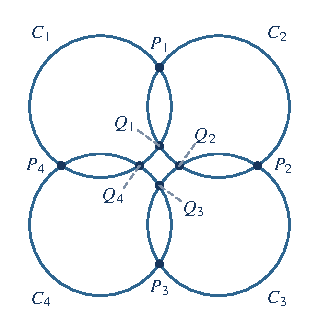
\includegraphics[width=.60\linewidth]{lb1-fig-01.pdf}
\FigureTag{LB1.1}{fig:lb1-01}
\end{figure}
This can be resolved using coordinates!
Now let us perform the magic; say with me these words: ``Problema invert\'o!''
% Source page 10 - right
Apply $I(P_1,R)$.
\begin{figure}[H]\centering
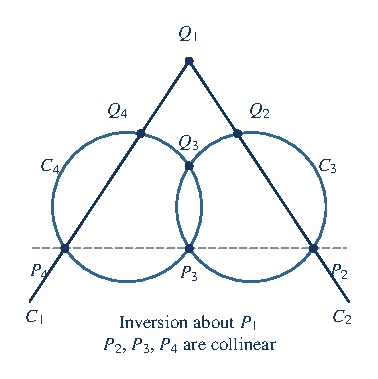
\includegraphics[width=.58\linewidth]{lb1-fig-02.pdf}
\FigureTag{LB1.2}{fig:lb1-02}
\end{figure}
Our magic worked! It remains to prove that $Q_1Q_2Q_3Q_4$ is concyclic.
Since $P_1P_2P_3P_4$ is concyclic, it inverts into a straight line; now $P_2,P_3,P_4$ are collinear.
It remains to chase three angles:
\[
\angle Q_3Q_4Q_1=\angle Q_3P_3P_4=\angle Q_3Q_2P_2
\Longrightarrow\angle Q_1Q_4Q_3=\angle Q_3Q_2P_2.
\]
This implies that $Q_1Q_2Q_3Q_4$ is concyclic. ``Finished!''

\setcounter{theorem}{30}\begin{lemma}[Distance formula for inversion]
If segment $AB$ inverts to $A_1B_1$ under $I(O,r)$, then
$A_1B_1=\dfrac{AB\,r^2}{OA\cdot OB}$.
\end{lemma}
This is helpful: it gives a two-line proof of Ptolemy's theorem.
\begin{figure}[H]\centering
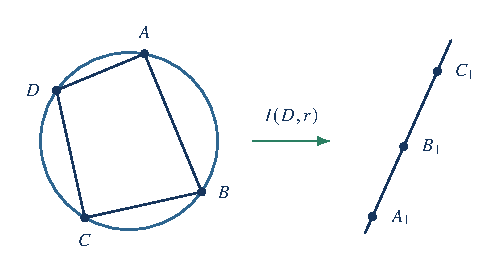
\includegraphics[width=.71\linewidth]{lb1-fig-03.pdf}
\FigureTag{LB1.3}{fig:lb1-03}
\end{figure}
% Source page 11 - left
I thought the proof would fit on the previous page, but it did not. Overconfidence is lethal!
From $A_1C_1=A_1B_1+B_1C_1$, inversion about $D$ gives
\[
\frac{AB\,r^2}{DA\cdot DB}+\frac{BC\,r^2}{DB\cdot DC}
=\frac{AC\,r^2}{DA\cdot DC}.
\]
Cancelling $r^2$ and multiplying through,
\[
\frac{AB\cdot CD+BC\cdot AD}{DA\cdot DB\cdot DC}
=\frac{AC}{DA\cdot DC}
\Longrightarrow AB\cdot CD+BC\cdot AD=AC\cdot BD.
\]

\setcounter{theorem}{31}\begin{lemma}[Similar triangles and concyclicity]\label{lemma:lb1-37}
If triangles $ABC$ and $AB'C'$ are similar, then $BB'CC'$ is concyclic.
\end{lemma}
This is an obvious geometric fact; a simple angle chase yields the result.
% Author check: vertex correspondence/orientation restrictions are not recorded.

\setcounter{theorem}{32}\begin{lemma}[Converse of the alternate-segment theorem]
An Olympiad student knows the alternate-segment theorem, but its converse is a powerful tool: the ``CAST lemma''.
\end{lemma}
The IMO jury loves posing problems where one is expected to show that a segment is tangent to a circle.
Instead of drawing the circle, if a simple angle chase establishes the converse of the alternate-segment theorem, ``that would be it!''
Let me show a lovely IMO problem resolved by a clever application of the above two lemmas.
In fact, I checked the competition papers: more than a dozen problems are of this type, and one appeared in IMO 2014!
% Source page 11 - right
\begin{figure}[H]\centering
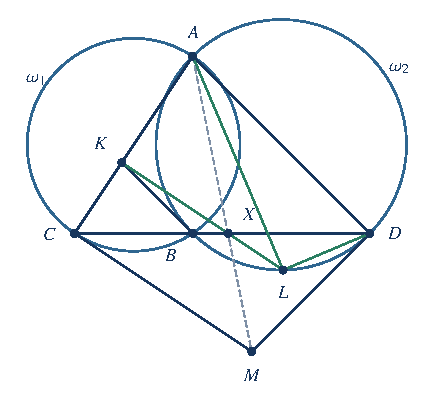
\includegraphics[width=.72\linewidth]{lb1-fig-04.pdf}
\FigureTag{LB1.4}{fig:lb1-04}
\end{figure}
Two circles intersect at $A$ and $B$. An arbitrary line through $B$ meets the first circle at $C$ and the second at $D$.
The tangents to $\omega_1$ at $C$ and to $\omega_2$ at $D$ meet at $M$.
Let $AM\cap CD=X$. Through $X$, a line parallel to $CM$ meets $AC$ at $K$.
Prove that $BK$ is tangent to the second circle.

We have $\angle BCM=\angle CAB$ and $\angle BDM=\angle BAD$.
Hence $\angle CAD=\angle BCM+\angle BDM=180^\circ-\angle CMD$, so $ACMD$ is concyclic.
Also $\angle DXL=\angle DCM=\angle CAB=\angle KXB$, giving
$\triangle ABC\sim\triangle XKC$ (AAA).
By Lemma~\ref{lemma:lb1-37}, $KBXA$ is cyclic.
Further, $\angle XCM=\angle KAB$ and $\angle CXM=\angle BKA$, so
$\triangle BKA\sim\triangle MXC$ (AAA).
Thus $\angle CMX=\angle KBA=\angle BDA$, and the CAST lemma gives the result.
% Author check: L appears in the drawing and proof without a textual definition; proof labels retained.

\subsection{Radical-axis theorem}
Let us begin by defining what is meant by the power of a point.
The idea was first discovered by ancient Greeks; Euclid wrote it in his \textit{Elements}.
The name ``power of a point'' (P.O.P.) was given by the world-renowned geometer Jacob Steiner.
\setcounter{theorem}{81}\begin{lemma}[Power of a point]\label{lemma:lb1-84}
Given a circle and a point $P$, draw a line through $P$ intersecting the circle at $A$ and $B$.
Then the product $PA\cdot PB$ stays constant.
\end{lemma}
\setcounter{theorem}{82}\begin{lemma}[Radical-axis theorem I]\label{lemma:lb1-85}
The locus of points whose powers with respect to two nonconcentric circles are equal is a line perpendicular to the line of centres of the two circles.
\end{lemma}
\setcounter{theorem}{83}\begin{lemma}[Radical-axis theorem II]\label{lemma:lb1-86}
If there are three circles $\omega_1,\omega_2,\omega_3$, then their radical axes are concurrent.
That point of concurrence is called the radical centre.
\end{lemma}
% Author check: no qualifications on the three circles or the possibility of parallel/undefined radical axes are stated.
Application 2 of Lemma 49 in the manuscript is immediate once you are aware of such a thing!
\paragraph{Application: USAMO (1997), problem 2.}
Let $ABC$ be a triangle, and draw isosceles triangles $DBC$, $AEC$, and $ABF$ external to $ABC$, with $BC$, $CA$, and $AB$ as their respective bases.
Prove that the lines through $A,B,C$ perpendicular to $EF,FD,DE$, respectively, are concurrent.
(There are 25 solutions to this problem!)
% Source page 43 - left
\begin{figure}[H]\centering
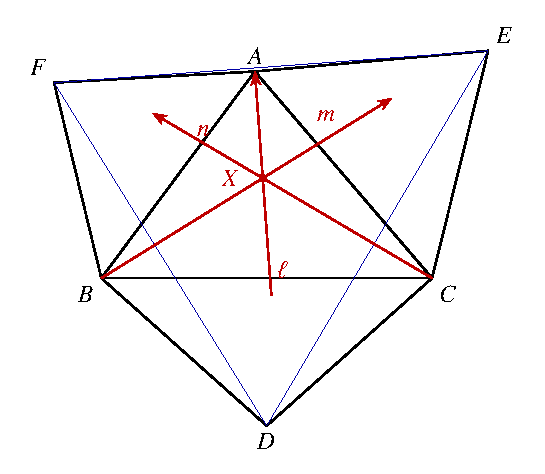
\includegraphics[width=.73\linewidth]{lb1-fig-21.pdf}
\FigureTag{LB1.21}{fig:lb1-21}
\end{figure}
It must be clear that we should somehow show $X$ to be the radical centre of three circles.
But where are the circles? Okay, be patient!
We have $\ell\perp EF$. In order for $\ell$ to be a radical axis, we must prove---no, not prove: construct---circles with centres $F,E$.
So let's exploit the fact that $FA=FB$ and $EA=EC$ by erecting circles with centres $F,E$ and radii $FA,EA$, respectively.
Argue similarly for point $D$, and don't forget to write Q.E.D.!

\paragraph{W.A.L.L.: What a Lovely Locus problem (I. F. Sharygin).}
Given a point $A$ inside a circle, construct a chord $XY$ passing through $A$.
Draw tangents at $X,Y$, and let their intersection be $P$. Find the locus of $P$. (Rephrased.)
Let $\omega$ be our circle, with centre $O$ and radius $r$, and let $A$ be a point inside it.
Construct a circle with diameter $AO$.
% Source page 44 - right
Given any chord $XY$ passing through $A$, its midpoint lies on this circle, since $\angle OBA=\angle OBX=90^\circ$ and $O$ is the centre.
\begin{figure}[H]\centering
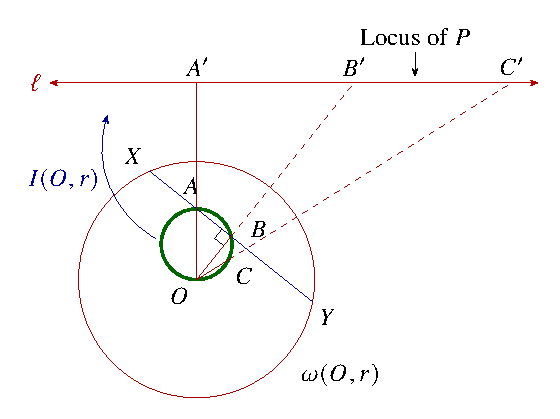
\includegraphics[width=.74\linewidth]{lb1-fig-22.pdf}
\FigureTag{LB1.22}{fig:lb1-22}
\end{figure}
Our point $P$ is nothing but the midpoint of the chord inverted with respect to $I(O,r)$.
Since a circle inverts back to a line, that line is precisely the locus---W.A.L.L.---of $P$.
Q.E.D.!
% Author check: the source does not exclude A=O or diameter chords, for which the tangent intersection is not a finite point.

\setcounter{theorem}{88}\begin{lemma}[Simson's line]\label{lemma:lb1-91}
The feet of the perpendiculars drawn from any point on the circumcircle of a triangle to its sides are collinear.
The converse is also true.
\end{lemma}
\paragraph{Application.}
The sides $AB,BC,AC$ of $\triangle ABC$ are cut by a transversal at $Q,R,S$, respectively.
The circumcircles of $\triangle ABC$ and $\triangle SCR$ intersect at $P$.
Prove that $ASPQ$ is cyclic.
% Source page 51 - left
\begin{figure}[H]\centering
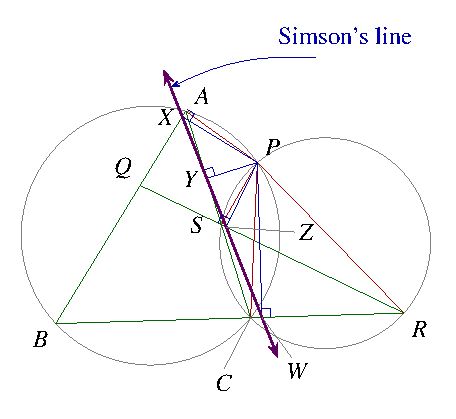
\includegraphics[width=.74\linewidth]{lb1-fig-27.pdf}
\FigureTag{LB1.27}{fig:lb1-27}
\end{figure}
Draw $PX,PY,PZ,PW$ perpendicular to $AB,AC,QR,BC$, respectively, as shown in the figure.
Since $P$ is on the circumcircle of $\triangle ABC$, the points $X,Y,W$ are collinear.
Since $P$ is on the circumcircle of $\triangle SCR$, the points $Y,Z,W$ are collinear.
It follows that $X,Y,Z$ are collinear. Thus $P$ lies on the circumcircle of $\triangle AQS$, and $APQS$ is cyclic.
Q.E.D.
\setcounter{theorem}{89}\begin{lemma}[Nine-point circle]\label{lemma:lb1-92}
The midpoints of the sides, the feet of the altitudes, and the midpoints of the segments joining the orthocentre to the vertices all lie on a circle, called the nine-point circle.
\end{lemma}
\paragraph{Application: Proofathon geometry contest (2014).}
In $\triangle ABC$, with orthocentre $H$, let $BH,CH$ intersect $AC,AB$ at $E,F$, respectively.
The tangent to the circumcircle of $\triangle ABC$ at $A$ intersects $BC$ at $P$.
Let $M$ be the midpoint of $AH$, and let $EF$ intersect $BC$ at $G$.
Prove that $PM\parallel GH$. (Draw that bullshit figure for yourself!)
% Source page 51 - right
By the nine-point-circle theorem, $DFME$ is cyclic, so $FX\cdot XE=DX\cdot MX$.
Also $HEAF$ is cyclic, since $\angle AFC=\angle AEH=90^\circ$, so $FX\cdot XE=XH\cdot XA$.
Therefore
\[\frac{FX\cdot XE}{FX\cdot XE}=\frac{DX\cdot MX}{XH\cdot HA}
\quad\Longrightarrow\quad\frac{DX}{XA}=\frac{XH}{MX}
\quad\Longrightarrow\quad\frac{HD+HX}{AM+MX}=\frac{HX}{MX}.\]
Thus $HD/AM=HX/MX$, and $HD/MH=HX/MX=DX/XA$, since $AM=MH$.
We have $PA^2=PB\cdot PC$ because $PA$ is tangent to the circumcircle of $\triangle ABC$.
Hence $PA/PB=PC/PA$, so $\triangle PAB\sim\triangle PCA$, and
$\angle PBA=\angle PCA=\angle BFC+\angle FCB$.
It follows that $\angle PBA=\angle BEC+\angle FEB=\angle GEC$, since $BFEC$ is cyclic.
Now $\angle PAC=\angle GEC$, so $GE\parallel PA$, and
\[\frac{GD}{PG}=\frac{DX}{XA}=\frac{HX}{MX}=\frac{HD}{MH},
\qquad\frac{GD}{PG}=\frac{HD}{MH},\]
giving $GH\parallel PM$.
Q.B.D.: Quite Boringly Done!
% Author check: D and X are used without definition in this source proof. The denominator XH*HA and angle claims are transcribed as written, not silently replaced by XA or other angles.
\setcounter{theorem}{90}\begin{lemma}[Excentre]\label{lemma:lb1-93}
The external bisectors of two angles and the internal bisector of the third concur at a point, called the excentre.
\end{lemma}
\paragraph{Application.}
In a triangle $ABC$, the lines formed by reflecting $BC$ across $AB$ and $AC$ intersect at $D$.
Prove that the circumcentre of $\triangle ABC$ lies on the circumcircle of $\triangle BCD$.
There is one more problem: take this one as an application of Ravi substitutions.
The bisector of $\angle A$ intersects $BC$ and the circumcircle of $\triangle ABC$ at $D,E$.
Show that $\triangle BDE$ and $\triangle CDE$ have the same circumradius.

% Source page 52 - left (rotated notebook page: Proofathon problem 3)
\paragraph{Proofathon, problem 3.}
The incentre of $\triangle BCD$ lies on the circumcentre of $\triangle ABC$.
Claim: try to prove this!
\begin{figure}[H]\centering
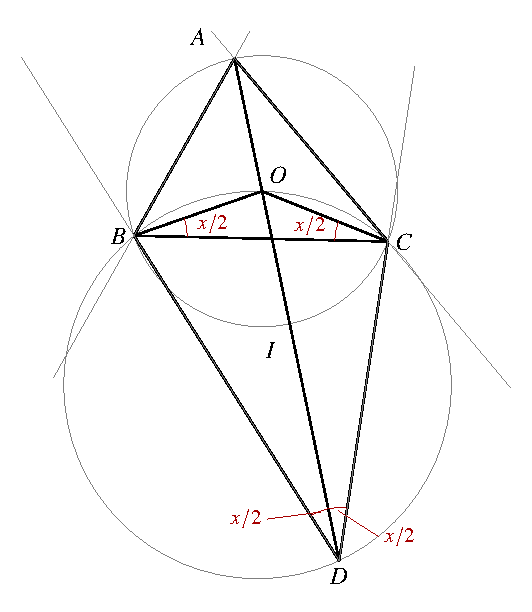
\includegraphics[width=.73\linewidth]{lb1-fig-28.pdf}
\FigureTag{LB1.28}{fig:lb1-28}
\end{figure}
\emph{Solution.} Join $AD$, and let it intersect the circumcircle of $\triangle BCD$ at $O$.
Now $BOCD$ is cyclic, so $\angle BOC=180^\circ-\angle BDC=180^\circ-x$.
Observe that $AB,AC$ are external angle bisectors of $\angle B,\angle C$ of $\triangle BCD$.
External bisectors of two angles and the internal bisector of the third are always concurrent.
Hence $AD$ is an angle bisector. Call this I.
From I, $\angle BDO=\angle CDO=x/2$, so $\angle OBC=\angle ODC=x/2$ and $\angle OCB=\angle ODB=x/2$.
Thus $\triangle BOC$ is isosceles, and $BO=OC$.
\paragraph{Crucial angle chase.}
We have $\angle ABC=90^\circ-\angle DBC/2$ and $\angle ACB=90^\circ-\angle DCB/2$.
Therefore
\[\angle BAC=180^\circ-\left(180^\circ-\frac{\angle DBC+\angle DCB}{2}\right)
=\frac{\angle DBC+\angle DCB}{2}=\frac{180^\circ-x}{2}=90^\circ-\frac x2.\]
Call this II. From II, $\angle BAC=90^\circ-x/2$, so $\angle BOC=2\angle BAC$, and also $OB=OC$.
Therefore $O$ is the circumcentre of $\triangle ABC$. Q.E.D.
% Author check: the introductory incentre/circumcentre wording is retained as written; the proof establishes a different claim and its final centre identification is left as in the source.
% Source page 52 - right (rotated notebook page: Proofathon problem 4)
\paragraph{Proofathon, problem 4.}\leavevmode\par
\begin{figure}[H]\centering
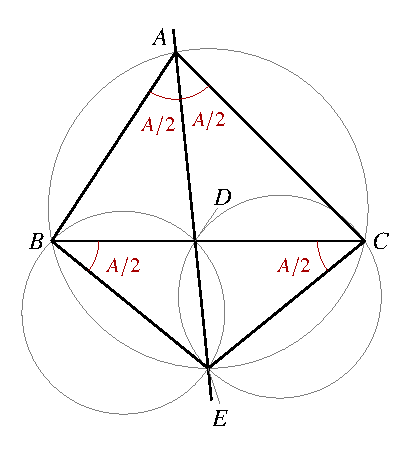
\includegraphics[width=.70\linewidth]{lb1-fig-29.pdf}
\FigureTag{LB1.29}{fig:lb1-29}
\end{figure}
We have $ABEC$ cyclic. Thus $A/2=\angle BCE=\angle BAD$, and $\angle CBE=\angle CAD=A/2$.
Since $AD$ bisects $\angle A$, we get $\angle BCE=\angle CBE=A/2$.
Hence $\triangle BEC$ is isosceles, so $BE=CE$; call this $\star$.
\paragraph{Facts.}
$R=abc/(4\Delta)$, where $\Delta$ is the area;
$\sin\theta=\sin(180^\circ-\theta)$; and $[ABC]=\tfrac12ab\sin\angle A$.
We have
\[R(\triangle BDE)=\frac{BD\cdot DE\cdot BE}{4[BDE]},
\qquad R(\triangle CDE)=\frac{DE\cdot CE\cdot DC}{4[CDE]}.\]
We seek $BD\cdot DE\cdot BE/(4[BDE])=DE\cdot CE\cdot DC/(4[CDE])$; call this I.
Since $BE=CE$, this reduces to $BD/[BDE]=CD/[CDE]$, or $BD/CD=[BDE]/[CDE]$.
Now
\[[BDE]=\tfrac12BD\cdot DE\sin\angle BDE,
\qquad[CDE]=\tfrac12DE\cdot CD\sin\angle CDE.\]
Consequently
\[\frac{[BDE]}{[CDE]}=
\frac{\tfrac12BD\cdot DE\sin\angle BDE}{\tfrac12DE\cdot CD\sin\angle CDE}
=\frac{BD}{CD},\]
because $\angle BDE=180^\circ-\angle CDE$.
This establishes I, hence $R(\triangle BDE)=R(\triangle CDE)$.
\emph{GeoGebra.}
% Source scan: some left-margin formula prefixes on this rotated page are clipped; the readable displayed repeated equality fixes their unambiguous continuation.

\paragraph{Magic of the nine-point circle: INMO (2012).}
Let $ABC$ be acute, and take $D,E,F$ on $BC,CA,AB$ so that $AD$ is a median,
$BE$ is the internal angle bisector, and $CF$ is an altitude.
Suppose $\angle FDE=\angle C$, $\angle DEF=\angle A$, and $\angle EFD=\angle B$.
Prove that $ABC$ is equilateral. Try it first!
% Source page 7 - right
\paragraph{Step 1.}
\begin{figure}[H]\centering
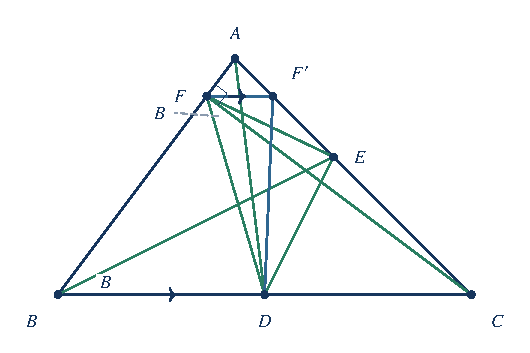
\includegraphics[width=.70\linewidth]{lb2-fig-05.pdf}
\FigureTag{LB2.5}{fig:lb2-05}
\end{figure}
Since $\angle AFD=\angle B+\angle FDB$, we obtain
$\angle AFE+\angle B=\angle B+\angle FDB$, so $\angle AFE=\angle FDB$.
Similarly $\angle AFE=\angle FDB=\angle DEC$.
Construct $FF'\parallel BC$. Then
$\angle F'FD=\angle FDB=\angle DEC$, so $FF'ED$ is cyclic.
\paragraph{Step 2.}
\begin{figure}[H]\centering
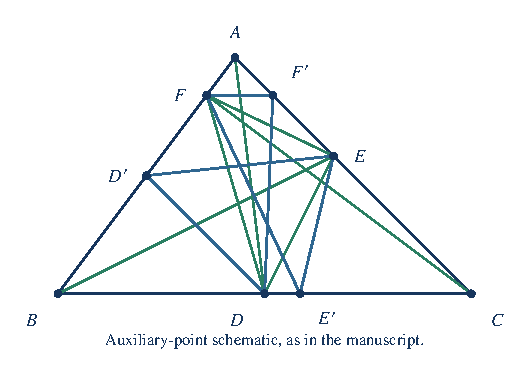
\includegraphics[width=.72\linewidth]{lb2-fig-06.pdf}
\FigureTag{LB2.6}{fig:lb2-06}
\end{figure}
A similar argument puts $F,F',E,E',D,D'$ on a circle.
Since $D$ is the midpoint of $BC$, $D'$ the midpoint of $AB$, and $F$ a perpendicular foot,
this is the nine-point circle. Wow!
The nine-point circle meets $AC$ at the perpendicular foot and the midpoint.
Thus $E$ is one of those two. Since $BE$ bisects the angle, this forces $AB=BC$; hence $E'$ and $D$ coincide.
Now $DE\parallel AB$, so $\angle DEC=\angle A$.
Step 1 gives $\angle FDB=\angle DEC=\angle A$.
Also $BD=CD$ and $\angle BFC=90^\circ$, so $FD=BD$ and $\angle DFB=\angle B$.
\paragraph{Step 3.}
In triangle $FDB$, $\angle B+\angle B+\angle A=180^\circ$.
In triangle $ABC$, $\angle B+\angle A+\angle A=180^\circ$.
Thus $2\angle B+\angle A=2\angle A+\angle B$ and $A=B=C=60^\circ$.
% Author check: auxiliary E',D' are introduced via the drawing; the argument presumes distinct circle intersections.

% Source page 8 - left
Here is another problem.
In triangle $ABC$, altitudes $BE,CF$ meet at $H$. Let $AM$ be a median and $HP\perp AM$.
Prove that $EF,PH,BC$, extended as necessary, are concurrent.
\begin{figure}[H]\centering
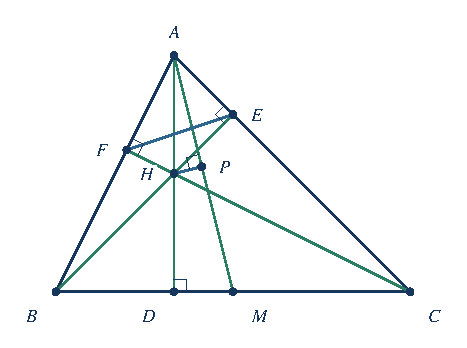
\includegraphics[width=.73\linewidth]{lb2-fig-07.pdf}
\FigureTag{LB2.7}{fig:lb2-07}
\end{figure}
This has a magical one-line solution. Try it and return!
Construct $AH\perp BC$ at $D$.
The sets $AFHPE$, $HPDM$, and $FEMD$ are each concyclic.
$EF$ is the radical axis of the first circle and the nine-point circle;
$HP$ is the radical axis of the first and second circles;
$DM$ is the radical axis of the second and the nine-point circle.
The radical-axis theorem gives the conclusion.
% Author check: special/parallel radical-axis configurations are not discussed.

\setcounter{theorem}{106}\begin{lemma}[The arc midpoint and the incentre]
In the configuration of Figure~\ref{fig:lb2-14}, $MI=MB=MC$.
\end{lemma}
\begin{figure}[H]
\centering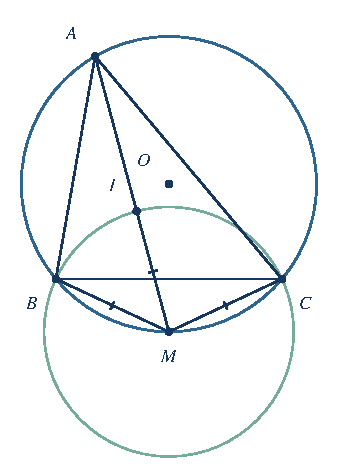
\includegraphics[width=.58\linewidth]{lb2-fig-14.pdf}
\FigureTag{LB2.14}{fig:lb2-14}
\end{figure}
\paragraph{Application: IMO 2006.}
Let $ABC$ have incentre $I$, and let $P$ be an interior point satisfying
$\angle PBA+\angle PCA=\angle PBC+\angle PCB$.
Show that $AP\geq AI$, with equality if and only if $P=I$.
This can be taken as an exercise: it is trivial once you notice that $BPIC$ is cyclic!
% BLOG-CONTENT-END
\end{document}
